\documentclass[cic,tc,english]{iiufrgs}

\usepackage[utf8]{inputenc}
\usepackage{graphicx}
\usepackage{times}
% \usepackage{palatino}
% \usepackage{mathptmx}       % p/ usar fonte Adobe Times nas fórmulas

\usepackage[alf,abnt-emphasize=bf]{abntex2cite}

\usepackage{lipsum}

\usepackage{revisornotes}
\usepackage{draftenvironment}

\usepackage{ragged2e}

\usepackage{listings}

\usepackage{amsmath}      % For math symbols
\usepackage[boxed]{algorithm}    % For the algorithm environment
\usepackage{algpseudocode} % For pseudocode formatting
\usepackage{xcolor}       % Optional for colored comments

\usepackage{tikz}

\usepackage{amsfonts}

\usepackage[bottom]{footmisc}

\usepackage{amssymb}

\title{
    A Hybrid Multi-Authority Attribute-Based Encryption scheme implementation for securing hIoT data
}
\translatedtitle{
    Um Esquema Híbrido de Criptografia Baseada em Atributos de Múltiplas Autoridades para Transmissão Segura de Dados hIoT
}

\author{Graeff}{Felipe de Almeida}

\advisor[Prof.~Dr.]{Nobre}{Jéferson Campos}
\coadvisor[M.Sc]{Soares}{Laura Rodrigues}

% \date{maio}{2001}
% \location{Itaquaquecetuba}{SP}

\keyword{cryptographic algorithms}
\keyword{IPFS}
\keyword{decentralized technologies}
\keyword{performance analysis}
\keyword{security evaluation}
\keyword{data storage}
\keyword{data exchange}

\translatedkeyword{algoritmos criptográficos}
\translatedkeyword{IPFS}
\translatedkeyword{tecnologias descentralizadas}
\translatedkeyword{análise de desempenho}
\translatedkeyword{avaliação de segurança}
\translatedkeyword{armazenamento de dados}
\translatedkeyword{intercâmbio de dados}

%\settowidth{\seclen}{1.10~}

\begin{document}

\maketitle

% dedicatory
\clearpage
\begin{flushright}
    \mbox{}\vfill
    \begin{tabular}{p{0.55\linewidth} p{0.45\linewidth}}
        In loving memory of Professor Raul Fernando Weber, a remarkable educator and influential figure in the field of computer security. His passion for teaching and dedication to his students left an indelible mark on all who had the privilege to learn from him. As I embark on my undergraduate thesis in computer security, I humbly dedicate this work to the memory of a great professor and a charismatic person who inspired generations of students, including myself. His guidance and enthusiasm ignited my love for this area, and I am forever grateful for the knowledge and inspiration he shared. His legacy lives on in the pursuit of knowledge and excellence. Rest in peace, \mbox{Professor} Weber.\\
    \end{tabular}
\end{flushright}

\chapter*{Acknowledgements}
    I would like to express my gratitude to my advisor, Professor Jéferson Campos Nobre, for his guidance and expertise throughout my research journey. His patience and profound knowledge have incentivised me to pursue this area of research.

    I am immensely thankful to Laura, whose foundational research laid the groundwork for this thesis. Her dedication and help have significantly contributed to the success of this project.

    My appreciation also extends to the faculty and staff at the Informatics Department. The education and support provided by the professors have been fundamental to my academic and professional growth. Their dedication to creating a nurturing and challenging academic environment has been critical to my development.

    Special thanks go to Valéria, my best friend, for her constant support and love. Her encouragement has been a pillar of strength in difficult times, reminding me of the value of perseverance.

    I am grateful to all my friends for their continued encouragement and belief in my abilities. Their support and the occasional much-needed distractions have helped me maintain my focus and passion for my research.

    Finally, I would like to thank Marina and Pedro, my psychologist and psychiatrist. Their professional support has been crucial in managing the stress of my academic commitments, significantly contributing to my well-being and success.

    This thesis reflects the collective support and encouragement of all those mentioned and many others, to whom I am deeply thankful.

\clearpage
\begin{flushright}
    \mbox{}\vfill
    \begin{minipage}{0.49\textwidth}
        % \setlength{\baselineskip}{1.2em} % Adjust line spacing
        \justifying
        \noindent
        {\itshape
        ``That is what I have always understood to
        be the essence of anarchism: the conviction
        that the burden of proof has to be placed on 
        authority, and that it should be dismantled 
        if that burden cannot be met.''\\
        }
        
        \raggedleft
        \parbox{\linewidth}{--- \textsc{Noam Chomsky,} \textit{Red and Black Revolution, No. 2} (May 1995)}
    \end{minipage}
\end{flushright}


\begin{abstract}
    \lipsum[1]
\end{abstract}

\begin{translatedabstract}
    \lipsum[1]
\end{translatedabstract}

\listoffigures

\listoftables

\listofalgorithms

\begin{listofabbrv}{MA-ABE} % longest abbreviation
    \item[AES] Advanced Encryption Standard
    \item[API] Application Programming Interface
    \item[DLP] Discrete Logarithm Problem
    \item[CBC] Cipher Block Chaining
    \item[ECC] Elliptic Curve cryptography
    \item[ECDLP] Elliptic Curve Discrete Logarithm Problem
    \item[EHR] Electronic Health Record
    \item[EMR] Electronic Medical Record
    \item[HIoT] Health Internet of Things
    \item[IoMT] Internet of Medical Things
    \item[IPFS] InterPlanetary File System
    \item[JSON] JavaScript Object Notation
    \item[MA-ABE] Multi-Authority Attribute-Based Encryption
    \item[NIST] National Institute of Standards and Technology
    \item[PoS] Proof of Stake
    \item[PoW] Proof of Work
    \item[REST] Representational State Transfer
    \item[RSA] Rivest-Shamir-Adleman
    \item[SHA] Secure Hash Algorithm
    \item[SIFF] Secure Identity Federation Framework
    \item[WSGI] Web Server Gateway Interface
\end{listofabbrv}

\begin{listofsymbols}{$\alpha\beta\pi\omega$}
    \item[$E_{K_{G_T}}$] Encrypted element $K_{G_T}$
    \item[$E_{\text{payload}}$] Encrypted payload data
    \item[$K_A$] Authorities' public keys
    \item[$K_{G_T}$] Element in the pairing group $G_T$
    \item[$K_{\text{SHA}}$] Hashed symmetric key
    \item[$K_{\text{user}}$] User attribute keys
\end{listofsymbols}

\tableofcontents

\clearpage
\ToDo{
    \begin{itemize}
        \item[$\boxtimes$] Terminar testes de tamanho de chave e tamanho de payload criptografado
        \item[$\square$] Colocar todas as abreviações na lista de abreviações
        \item[$\square$] Colocar abreviações por extenso somente na primeira ocorrência
        \item[$\square$] Reescrever a seção de Related Works 
        \item[$\square$] Incrementar proposed solution
    \end{itemize}
}

\chapter{Introduction}
    \label{chap:introduction}
    % contextualização 1
    \begin{draft}{Talk about lauras paper}
        Laura's paper ...
        \ToDo{Perguntar pra Laura em que camada do framework dela entra a criptografia}    
    \end{draft}


    % contextualização 2 - mais especificacao
    \begin{draft}{Talk specifities about the technologies used in the framework and why security is relevant and not adressed by IPFS and Hyperledger}
        IPFS \cite{benet2013ipfs} is a peer-to-peer (P2P) decentralized storage system based on a content-addressable block storage model.
    \end{draft}

    % trabalhos relacionacios
    \begin{draft}{Talk about related works}
        
    \end{draft}

    \begin{draft}{Gap}
        No entanto, nenhum dos trabalhos ...
    \end{draft}

    % proposta

    In the present thesis, we aim to propose a cryptography framework that best fits the solution introduced by \citet{laura2023}.

    % (opcional) avaliação (implementação, experimentos, resultados)

    \begin{draft}{Quick introduction of each chapter}
        In Section \ref{chap:relatedworks},...

    \end{draft}

\chapter{Background}
    \label{chap:background}

    \citet{laura2023} proposed a new framework for securing Health Internet of Things (HIoT) data. The framework aims to provide a secure and decentralized storage solution for HIoT data using InterPlanetary File System (IPFS) \cite{benet2013ipfs} for decentralized storage and Hyperledger Fabric \cite{fabric} for access control and data management. However, the framework lacks a robust cryptographic solution to ensure data confidentiality, data ownership, access control, and privacy. We extend their framework by proposing a hybrid cryptographic approach to enhance the security of the system and enable fine-grained access control based on user attributes.

    In this work, the key generation and encryption processes adopt a hybrid cryptographic approach that combines elliptic curve cryptography (ECC), pairing-based cryptography (PBC), and symmetric encryption using the Advanced Encryption Standard (AES). The system implements a Multi-Authority Attribute-Based Encryption (MA-ABE) scheme, enabling fine-grained and flexible access control based on user attributes distributed across multiple independent authorities. ECC and PBC provide the foundation for secure key establishment and attribute-based policies, while AES ensures efficient encryption of large data volumes. This combination leverages the strengths of each technique to achieve both performance and robust access control.



    Section~\ref{sec:ecc} provides an overview of elliptic curve cryptography, including the definition of elliptic curves and their use in cryptographic systems. Section~\ref{sec:pairing} introduces pairing-based cryptography and its applications in advanced cryptographic constructions. Section~\ref{sec:maabe} describes Multi-Authority Attribute-Based Encryption (MA-ABE) and its benefits for secure data sharing in decentralized systems. Section~\ref{sec:symmetric} presents the Advanced Encryption Standard (AES) and its role in symmetric encryption. Section~\ref{sec:blockchain} discusses the application of blockchain technology in healthcare and its potential to enhance data security and privacy. Further details on how these cryptographic techniques are integrated into the proposed framework are provided in Chapter~\ref{chap:proposedsolution}.
    

    \section{Elliptic Curve Cryptography}
        \label{sec:ecc}

        \citet{hankerson2004guide} define Elliptic Curve Cryptography (ECC) as a public-key cryptosystem based on the algebraic structure of elliptic curves over finite fields. Its security relies on the difficulty of the Elliptic Curve Discrete Logarithm Problem (ECDLP), which is believed to be computationally infeasible to solve in general-purpose cases~\citep{hankerson2004guide, koblitz1987elliptic}.

        Let $p$ be a prime number, and let $\mathbb{F}_p$ denote the finite field of integers modulo $p$. An elliptic curve $E$ over $\mathbb{F}_p$ is defined by the Weierstrass equation:

        \begin{equation}
        \label{eq:elliptic_curve}
        y^2 = x^3 + ax + b
        \end{equation}

        where $a, b \in \mathbb{F}_p$ are curve parameters chosen such that the curve is non-singular, i.e., $4a^3 + 27b^2 \neq 0$. The set of points $(x, y) \in \mathbb{F}_p^2$ satisfying this equation, together with a special point at infinity, form an abelian group under a well-defined addition operation~\citep{hankerson2004guide}.

    \section{Pairing-Based Cryptography}
        \label{sec:pairing}

        Pairing-based cryptography extends the use of elliptic curves by employing bilinear pairings, which are maps of the form:

        \begin{equation}
        e: G_1 \times G_2 \rightarrow G_T
        \end{equation}

        where $G_1$ and $G_2$ are additive cyclic groups of points on elliptic curves, and $G_T$ is a multiplicative cyclic group of a finite field~\citep{boneh2001identity}. The pairing $e$ satisfies the following properties:

        \begin{itemize}
            \item \textbf{Bilinearity}: $e(aP, bQ) = e(P, Q)^{ab}$ for all $P \in G_1$, $Q \in G_2$, and integers $a, b$.
            \item \textbf{Non-degeneracy}: There exist points $P \in G_1$ and $Q \in G_2$ such that $e(P, Q) \neq 1$.
            \item \textbf{Computability}: The pairing $e(P, Q)$ can be efficiently computed using algorithms such as Miller's algorithm~\citep{miller1986use}.
        \end{itemize}

        Pairings enable advanced cryptographic constructions, including identity-based encryption (IBE), attribute-based encryption (ABE) and short signatures~\citep{boneh2001identity}.

    \section{Multi-Authority Attribute-Based Encryption (MA-ABE)}
        \label{sec:maabe}
        Attribute-Based Encryption (ABE) is a cryptographic scheme that allows encryption and decryption operations based on user attributes rather than individual identities~\citep{goyal2006attribute}. In a Multi-Authority ABE (MA-ABE) model, multiple independent authorities manage disjoint sets of attributes, improving decentralization and resistance to single points of failure~\citep{chase2007multi}. Each authority issues keys corresponding to the attributes it controls, enabling fine-grained access policies defined over attributes from multiple domains.
        
        MA-ABE is particularly suitable for systems where sensitive data access must be controlled by multiple stakeholders, as is the case in healthcare scenarios. The combination with pairing-based cryptography enables efficient implementation of complex access policies.

        
    \section{Symmetric Encryption with AES}
        \label{sec:symmetric}
        The Advanced Encryption Standard (AES) is a symmetric block cipher standardized by the National Institute of Standards and Technology (NIST)~\citep{daemen1999aes}. It operates on fixed-size blocks of data (typically 128 bits) and supports key sizes of 128, 192, or 256 bits. AES is widely used for data confidentiality due to its efficiency and strong security guarantees.
        
        In this system, AES is used to encrypt large datasets stored off-chain, while the encryption keys are protected using the MA-ABE scheme. This hybrid design ensures both performance and access control granularity.
        
    \section{Blockchain Technology in Healthcare}
        \label{sec:blockchain}
        \begin{draft}{Laura vai escrever isso aqui}
        \end{draft}

\chapter{Related Works}
    \label{chap:relatedworks}

    This chapter reviews existing literature relevant to the secure management and sharing of data in Health Internet of Things (HIoT) environments. The pervasive nature of HIoT devices necessitates robust solutions for data confidentiality, integrity, and fine-grained access control. This review systematically categorizes and discusses prior research in cryptographic techniques and blockchain-based systems applied to healthcare. Critically, it contextualizes the foundational work by \citet{laura2023}, which proposed an architecture for storing hIoT data in IPFS and specifically identified the detailed cryptographic scheme and algorithms as a crucial direction for future research. This thesis undertakes that identified research opportunity. Furthermore, this chapter identifies current limitations and broader gaps in the literature that underscore the need for the hybrid cryptographic framework proposed herein.

    The chapter is structured as follows: Section~\ref{sec:overallcontext} provides an overall context of cryptographic and blockchain-based solutions in healthcare, highlighting key advancements. Section~\ref{sec:securedata} delves into specific approaches for secure data sharing and storage in hIoT environments, including the architectural foundation proposed by \citet{laura2023}. Finally, Section~\ref{sec:problemstatement} articulates the problem statement, identifying the gaps that this research aims to address.

    \section{Overall Context}
    \label{sec:overallcontext}

        This section provides an overview of existing research related to securing healthcare data, with a particular focus on broader cryptographic techniques and general blockchain-based solutions. The exponential growth of Health Internet of Things (HIoT) devices has led to an unprecedented volume of sensitive patient data, making robust security, privacy, and access control mechanisms paramount. We examine how various studies address these challenges, setting the stage for understanding the motivations and contributions of our proposed hybrid cryptographic framework.

        \subsection{Cryptographic Approaches for Healthcare Data Security}
            Securing sensitive healthcare data often relies on advanced cryptographic primitives to ensure confidentiality, integrity, and authenticity. However, designing and verifying the security of complex primitives such as Attribute-Based Encryption (ABE) is a recognized challenge in cryptography. Indeed, recent cryptanalysis efforts by \citet{broken2020} have demonstrated vulnerabilities in numerous ABE schemes, including several multi-authority variants, underscoring the critical need for rigorously analyzed and robust constructions. In this context, \citet{Memos2021} propose a layered cloud architecture that integrates Advanced Encryption Standard (AES) and Rivest-Shamir-Adleman (RSA) encryption to enhance the security of e-health data transmission. This highlights the use of hybrid encryption, similar to our approach, for efficient data protection. \citet{Hema2019} further assess ECC-based encryption mechanisms, showcasing their effectiveness in securing healthcare data within cloud environments. This directly relates to our use of ECC as a foundational element. More recently, \citet{Naz2024} explore defenses against emerging quantum computing threats in blockchain through exotic signatures, emphasizing the continuous need for cryptographic innovation in this domain.


        \subsection{Blockchain for Data Integrity and Secure Sharing}
            Blockchain technology offers a decentralized and immutable ledger, making it highly suitable for enhancing data integrity, transparency, and secure sharing in healthcare. Several works leverage blockchain to establish robust security frameworks. For instance, \citet{Tian2019} utilize the Secure Identity Federation Framework (SIFF) alongside Hyperledger Fabric to ensure the integrity, availability, and privacy of medical data. \citet{Esposito2018} investigate how blockchain can generally enhance data security in cloud-based healthcare systems, addressing inherent vulnerabilities in traditional centralized models. \citet{Rahman2020} describe a blockchain-based platform specifically designed for secure cross-border data sharing, aiming to build trust and enhance security across different jurisdictions. The use of Hyperledger Fabric for scalable solutions in securing IoT data is also explored by \citet{Eghmazi2024}.
    

    \section{Secure Data Sharing and Storing in hIoT}
        \label{sec:securedata}
        This section delves into specific architectural solutions for secure data sharing and storage within hIoT environments, focusing on approaches that integrate advanced cryptographic mechanisms with decentralized technologies. These works provide the direct context for the development of our proposed hybrid cryptographic framework.

        \subsection{IPFS hIoT Data Storage Framework and Foundational Architecture}
            \begin{draft}{Discuss the framework proposed by Laura}
            \end{draft}


        \subsection{Attribute-Based Access Control in Decentralized Healthcare Architectures}
            This subsection focuses on works that specifically integrate Attribute-Based Encryption (ABE) and Multi-Authority ABE (MA-ABE) into decentralized healthcare data architectures, which is central to our proposed solution. \citet{Guo2019Flexible} propose a flexible and efficient blockchain-based ABE scheme with multiple authorities tailored for medical on-demand services in telemedicine systems, focusing on independent key updates. Similarly, \citet{Ghaffaripour2019Cryptographically} investigate cryptographically enforced access control within blockchain platforms by incorporating ABE schemes to enhance privacy and broaden applicability. \citet{Jin2019Secure} introduce a comprehensive framework for secure, privacy-preserving, and interoperable medical data sharing that holistically integrates multi-authority ABE with blockchain and smart contracts to enforce sharing policies. Building on this, \citet{Yang2022Blockchain} propose a patient-controlled and cloud-chain collaborative multi-authority ABE scheme for EHR access control, supporting verifiable outsourcing decryption and hiding access policies. Further advancements include \citet{Li2023Secure}, who detail a secure blockchain-assisted MA-ABE scheme with keyword search for smart healthcare systems in fog computing, aiming for fine-grained access control and search functionality while reducing computation tasks. Moreover, \citet{Guo2023Hybrid} present a hybrid blockchain-edge architecture for EHR management, integrating MA-ABE with homomorphic encryption to protect patient anonymity and safeguard records. These works demonstrate the growing trend of embedding advanced ABE capabilities directly into distributed systems for granular and robust access control.

            Beyond these integrated approaches, other studies focus on the ABE schemes themselves within decentralized contexts. \citet{Zala2024} enhance e-health data privacy through an attribute-based encryption scheme that significantly improves anonymity, demonstrating the utility of ABE in protecting user identities. \citet{Bhansali2022} integrate ciphertext-policy attribute-based encryption with federated learning for data management in the Internet of Medical Things (IoMT), showcasing a practical application of ABE for managing access to sensitive health data. Additionally, \citet{Esfahani2024} introduce a comprehensive privacy scheme for IoT-based systems using zero-knowledge proofs and ring signatures, offering alternative methods for achieving granular privacy, and \citet{Li2024} contributes by creating a regulated medical data trading scheme that ensures privacy and compliance through blockchain and zero-knowledge proofs.

    \section{Problem Statement}
        \label{sec:problemstatement}

        The rapidly expanding landscape of Health Internet of Things (HIoT) generates vast quantities of sensitive patient data, demanding robust solutions for confidentiality, integrity, and access control within decentralized systems. While architectural frameworks, such as the one proposed by \citet{laura2023} utilizing IPFS for decentralized storage and Hyperledger Fabric for data management, lay a strong foundation, they often leave the critical details of cryptographic implementation for fine-grained data security as open challenges or future work. This thesis directly addresses these specific gaps.

        Despite these advancements, fully realizing the potential of secure hIoT data management necessitates further exploration into several key areas, which this thesis identifies as critical challenges, as detailed in the following subsections.

        \subsection{Absence of a Concrete Cryptographic Layer in Existing HIoT Architectures}
            Many proposed decentralized architectures for hIoT data, including the foundational framework by \citet{laura2023}, effectively address data decentralization and integrity through technologies like IPFS and blockchain. However, these frameworks typically lack a concrete, implemented cryptographic layer capable of providing end-to-end data confidentiality and fine-grained access control over the actual data payloads. Without such a layer, data stored on decentralized systems, while immutable and verifiable, remains vulnerable to unauthorized access if a user gains access to the storage location, failing to meet the stringent privacy requirements of healthcare.

        \subsection{Limited Fine-Grained Access Control in Multi-Stakeholder Environments}
            Traditional cryptographic methods (e.g., simple symmetric or public-key encryption) offer binary access control, which is insufficient for the complex, multi-stakeholder environment of hIoT. Healthcare scenarios demand dynamic and granular access rights based on user attributes (e.g., 'doctor,' 'researcher,' 'hospital'), not just individual identities. Existing solutions often struggle to efficiently manage and enforce such attribute-based policies across multiple independent authorities, leading to either cumbersome key management or inadequate security.

        \subsection{Performance and Scalability Challenges of Advanced Cryptographic Primitives}
            Implementing advanced cryptographic schemes, particularly those offering fine-grained access control like Attribute-Based Encryption (ABE), often introduces significant computational overhead. This overhead can hinder the performance and scalability of hIoT systems, which process high volumes of data from resource-constrained devices. Balancing the strong security guarantees of these primitives with the operational efficiency required for real-time hIoT applications remains a critical hurdle.

        \subsection{Verification and Robustness of Cryptographic Schemes}
            The complexity inherent in designing and implementing sophisticated cryptographic schemes, especially Multi-Authority ABE (MA-ABE), makes rigorous security verification challenging. As highlighted by cryptanalysis efforts, such as those by \citet{broken2020}, numerous published ABE schemes have been found to contain vulnerabilities. This underscores a persistent problem in the field: the difficulty in ensuring the practical robustness of schemes beyond their theoretical proofs. Consequently, there is a pressing need for carefully selected, robustly implemented, and practically evaluated cryptographic solutions to guarantee the trustworthiness of hIoT data security.

\chapter{Proposed Solution}
    \label{chap:proposedsolution}
    This chapter presents the proposed solution for enhancing the security of Health Internet of Things (HIoT) data storage and sharing. The approach integrates blockchain-based storage with a hybrid cryptographic scheme using Multi-Authority Attribute-Based Encryption (MA-ABE). The solution builds upon the framework proposed by \citet{laura2023}, addressing its lack of cryptographic mechanisms by incorporating a layered encryption strategy.

    The solution consists of a hybrid cryptographic approach that combines symmetric encryption for payload protection and MA-ABE for secure key distribution. This chapter focuses solely on the cryptographic mechanisms designed and implemented in this work.

    \section{Hybrid Multi-Authority Attribute-Based Encryption Scheme for Securing HIoT Data}
    \label{sec:encryption}

        This section presents the cryptographic core of the proposed solution, which uses a hybrid encryption scheme combining MA-ABE and symmetric encryption using AES. The goal is to achieve efficient, fine-grained access control for large hIoT payloads.

        \subsection{Overview of the Encryption and Decryption Workflows}
            The encryption process consists of the following stages:
            \begin{enumerate}
                \item Authorities are initialized and generate public/private key pairs.
                \item Users are assigned attributes and corresponding secret keys by the authorities.
                \item A symmetric key is randomly generated as an element of the pairing group $G_T$.
                \item The symmetric key is hashed with SHA-256 to derive an AES key.
                \item The payload is encrypted with AES.
                \item The original symmetric key is encrypted using MA-ABE under a specified attribute policy.
            \end{enumerate}

            The decryption process involves the following steps:
            \begin{enumerate}
                \item Users possess secret keys associated with their attributes, issued by different authorities.
                \item The encrypted symmetric key (an element of $G_T$) is decrypted using MA-ABE, if the user's attributes satisfy the access policy.
                \item The recovered element from $G_T$ is hashed with SHA-256 to derive the AES key.
                \item The payload is decrypted using AES with the derived key.
                \item The plaintext is unpadded to retrieve the original data.
            \end{enumerate}

            This ensures that only users who possess the required attributes can decrypt the MA-ABE-encrypted symmetric key and subsequently access the payload.


        \subsection{Key Management and Distribution}
            The key management system is designed to handle the generation, storage, and distribution of keys securely. Each authority generates its public/private key pair and distributes the public keys to users. The private keys are securely stored and used for generating user-specific keys based on their attributes.

        \subsection{Key Generation and Authority Setup}
            Authorities generate keys using the MaabeRW15 scheme from the Charm-Crypto library. Each authority is responsible for a disjoint subset of attributes and securely stores its private key. Public keys are distributed system-wide.

        \subsection{Access Policy Specification}
            Encryption policies are defined using boolean expressions over attributes, such as in the example policy~\ref{eq:policy_example}, where the attributes are specified in the format "<attribute>@<authority>". The policy can include AND, OR, and NOT operations to define complex access conditions. This allows for flexible and fine-grained access control based on user attributes.
            This policy structure allows flexible definitions of access, combining multiple authorities and domains.

            \begin{equation}
                \label{eq:policy_example}
                \texttt{(\allowbreak doctor@HOSPITAL \allowbreak AND \allowbreak researcher@UNIVERSITY) \allowbreak OR \allowbreak regulator@GOVERNMENT}
            \end{equation}


        \subsection{Security and Performance Considerations}
            This scheme ensures:
            \begin{itemize}
            \item \textbf{Fine-grained access control}: via MA-ABE policies.
            \item \textbf{Efficiency}: AES handles bulk data, reducing computational cost.
            \item \textbf{Scalability}: Multiple authorities reduce centralization and key distribution bottlenecks.
            \end{itemize}

            Further evaluation of performance and scalability is provided in Chapter~\ref{chap:evaluation}.


\chapter{Experimental Setup}
\label{chap:experimentalsetup}

    This chapter presents the algorithmic design of the proof-of-concept implementation based on the cryptographic Here, we detail the key routines responsible for authority initialization, attribute-based key generation, and the hybrid encryption and decryption processes. Additionally, we include schematic illustrations and pseudocode to clarify the functional logic of each step.

    \section{Authority and Key Management}
    \label{sec:authority-key-management}

        This section details the setup and management of authorities and the generation of attribute-based keys within our implemented system. These foundational processes are critical for establishing the decentralized access control mechanism.

        \subsection{Authority Setup}

            Each authority is identified by a unique identifier and is responsible for managing a disjoint subset of attributes. During the setup phase, each authority generates a public and private key pair using a multi-authority attribute-based encryption scheme. The public key is made available to all clients, while the private key is securely stored and used later to issue attribute-based keys.

            \begin{algorithm}
                \caption{Setup Authority}
                \label{alg:setup_authority}
                \begin{algorithmic}[1]
                \Procedure{SetupAuthority}{authority}
                    \State $pk, sk \gets \textsc{generateAuthorityKeys}()$
                    \State $\textsc{storeAuthorityKeys}(authority, pk, sk)$
                \EndProcedure
                \end{algorithmic}
            \end{algorithm}

        \subsection{Attribute-Based Key Generation}
            Once an authority is initialized, it can issue secret key components to users based on their assigned attributes. Each key is generated using the authority's private key and the attribute identifier.

            \begin{algorithm}
                \caption{Key Generation}
                \label{alg:keygen}
                \begin{algorithmic}[1]
                \Procedure{Keygen}{authority, attribute, user}
                    \State $sk \gets \textsc{retrieveAuthorityPrivateKey}(authority)$
                    \State $K \gets \textsc{generateKey}(sk, attribute)$
                    \State $\textsc{storeKey}(user, K)$
                \EndProcedure
                \end{algorithmic}
            \end{algorithm}

    \section{Hybrid Encryption Workflow}
    \label{sec:encryption-workflow}
        This section describes the procedure used to encrypt a data payload using a hybrid approach that combines symmetric encryption with attribute-based access control. Access is restricted based on boolean expressions over user attributes.

        \begin{figure}[h]
        \centering
        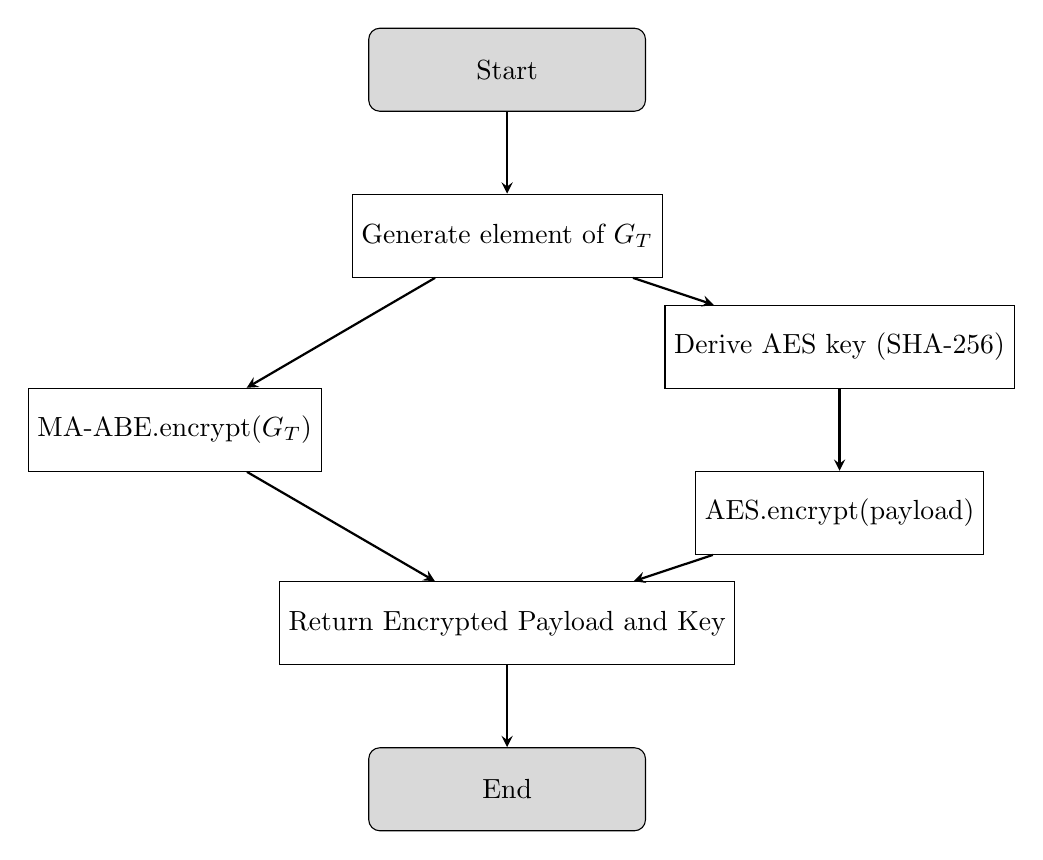
\begin{tikzpicture}[node distance=7em]
            \usetikzlibrary{positioning, fit}

            \tikzset{
                startstop/.style = {rectangle, rounded corners, minimum width=10em, minimum height=3em, text centered, draw=black, fill=gray!30},
                process/.style = {rectangle, minimum width=10em, minimum height=3em, text centered, draw=black, fill=white!30},
                arrow/.style = {thick,->,>=stealth}
            }

            \node (start) [startstop] {Start};
            \node (gt) [process, below of=start, node distance=6em] {Generate element of $G_T$};
            \node (sha) [process, below right of=gt, xshift=10em, yshift=-2em] {Derive AES key (SHA-256)};
            \node (aes) [process, below of=sha, node distance=6em] {AES.encrypt(payload)};
            \node (maabe) [process, below left of=gt, xshift=-10em, yshift=-5em] {MA-ABE.encrypt($G_T$)};
            \node (return) [process, below of=gt, node distance=14em] {Return Encrypted Payload and Key};
            \node (stop) [startstop, below of=return, node distance=6em] {End};

            \draw [arrow] (start) -- (gt);
            \draw [arrow] (gt) -- (sha);
            \draw [arrow] (gt) -- (maabe);
            \draw [arrow] (sha) -- (aes);
            \draw [arrow] (maabe) -- (return);
            \draw [arrow] (aes) -- (return);
            \draw [arrow] (return) -- (stop);
        \end{tikzpicture}
        \caption{Hybrid encryption process combining symmetric and attribute-based encryption}
        \label{fig:encrypt_process}
        \end{figure}

        \subsection{AES Key Derivation}

            A random element is first generated in the bilinear pairing group $G_T$. This element is then serialized and hashed using SHA-256 to obtain a 256-bit AES key.

            \begin{equation}
            \text{hashed\_key} = \text{SHA-256}(\text{serialized}(K_{G_T}))
            \end{equation}

        \subsection{Payload Encryption}

            The payload is padded to match the AES block size and encrypted using the derived key in CBC mode. Simultaneously, the original element in $G_T$ is encrypted using the attribute-based encryption scheme under a specified access policy.

            \begin{algorithm}
                \caption{Encryption Process}
                \label{alg:encryption_process}
                \scriptsize
                \begin{algorithmic}[1]
                \Procedure{Encrypt}{payload, policy}
                    \State $K_{G_T} \gets \textsc{Random}(G_T)$
                    \State $A \gets \textsc{getAuthorities}(\text{policy})$
                    \State $K_{\textsc{A}} \gets \textsc{retrievePublicKeys}(A)$
                    \State $K_{\textsc{SHA}} \gets \textsc{SHA256}(K_{G_T})$
                    \State $E_{K_{G_T}} \gets \textsc{maabe.Encrypt}(K_{\textsc{A}}, K_{G_T}, \text{policy})$
                    \State $E_{\text{payload}} \gets \textsc{AES.encrypt}(\text{payload}, K_{\textsc{SHA}})$
                    \State \Return $E_{K_{G_T}}, E_{\text{payload}}$
                \EndProcedure
                \end{algorithmic}
            \end{algorithm}

    \section{Decryption Workflow}
    \label{sec:decryption-workflow}

        To recover the original data, the user must possess the necessary set of attributes to satisfy the encryption policy.

        \begin{enumerate}
            \item The MA-ABE-encrypted key element is decrypted using the user's attribute-based secret keys.
            \item The resulting group element is hashed using SHA-256 to regenerate the AES key.
            \item The AES key is used to decrypt the payload.
            \item Padding is removed to retrieve the original data.
        \end{enumerate}

        \begin{algorithm}
            \caption{Decryption Process}
            \label{alg:decryption_process}
            \scriptsize
            \begin{algorithmic}[1]
            \Procedure{Decrypt}{$E_{K_{G_T}}$, $E_{\text{payload}}$, $K_{\text{user}}$}
                \State $K_{G_T} \gets \textsc{maabe.Decrypt}(E_{K_{G_T}}, K_{\text{user}})$
                \State $K_{\textsc{SHA}} \gets \textsc{SHA256}(K_{G_T})$
                \State $payload \gets \textsc{AES.decrypt}(E_{\text{payload}}, K_{\text{SHA}})$
                \State \Return $payload$
            \EndProcedure
            \end{algorithmic}
        \end{algorithm}





\chapter{Evaluation}
    \label{chap:evaluation}
    This chapter presents the implementation details and performance evaluation of the cryptographic system proposed in the previous chapters. We describe the technologies used, the deployment environment, the testing methodology, and the results obtained under different configurations. To ensure reproducibility of results, all source code developed for this project has been archived and made publicly available through Zenodo~\citep{maabeflask}.

    

    \section{Evaluation Strategy and Testbed}
        \label{sec:evaluation-setup}
        This section outlines the evaluation methodology and presents the test environment used to assess the performance of the implemented system. We begin by defining the evaluation objectives, then describe the hardware and software used. Finally, we introduce the tools and configurations employed during the experiments.

        \subsection{Evaluation Objectives}
        \label{subsec:evaluation-objectives}
            The main objectives of the evaluation are to measure the system's performance in terms of response time, determine its scalability under increasing workloads, and assess the cryptographic overhead introduced by the MA-ABE scheme. In addition, we aim to understand how the number of user attributes affects key size and to verify the security of the implementation.

        \subsection{Hardware and Software Environment}
        \label{subsec:hardware-software}
            The experiments were conducted on a single machine whose specifications are listed in Table~\ref{tab:machine_specs}. This section describes the hardware and operating system used, providing context for interpreting the performance results presented later in this chapter.


            \begin{table}[h]
                \centering
                \begin{tabular}{|l|l|}
                \hline
                \textbf{Component} & \textbf{Details} \\ \hline
                Operating System & Linux Mint 22.1 (x86\_64) \\ \hline
                Kernel Version & 6.8.0-57-generic \\ \hline
                Processor & AMD Ryzen 5 PRO 7640HS @ 5.015 GHz \\ \hline
                Architecture & x86\_64 (12 threads, 6 physical cores) \\ \hline
                Memory & 14 GiB RAM, 15 GiB swap \\ \hline
                Storage & NVMe SSD \\ \hline
                Python Version & 3.10.17 \\ \hline
                Containerization & Docker 28.0.4, Docker Compose v2.34.0 \\ \hline
                \end{tabular}
                \caption{Machine specifications and environment configuration used in testing}
                \label{tab:machine_specs}
            \end{table}
                

            
            \subsection{Implementation Tools}
            \label{subsec:tools}

                To evaluate the implementation of the proposed scheme, we used several tools and frameworks that support API development, cryptographic computation, concurrency management, and load testing.

                \textbf{Locust} is a Python-based API load testing tool that allows the definition of user behavior scenarios to simulate concurrent usage. It generates load on the system to evaluate responsiveness and performance under various conditions. We configured it with varying numbers of users and spawn rates to assess scalability.

                \textbf{Gunicorn} is a Web Server Gateway Interface (WSGI) server for Python applications. It enables concurrent request handling through configurable worker processes and threads. We varied the number of threads and workers to test different concurrency configurations and identify an optimal setup.

                \textbf{Charm-Crypto} is a Python library for pairing-based cryptography that offers high-level abstractions for implementing complex cryptographic protocols. It supports a variety of schemes, including Multi-Authority Attribute-Based Encryption (MA-ABE). In our implementation, we used the \emph{MaabeRW15} scheme proposed by Rouselakis and Waters~\citep{rouselakis2015efficient}, which provides efficient support for multi-authority setups. Charm-Crypto handled all cryptographic operations in our system.

                \textbf{Flask} is a lightweight web framework for Python used to implement the RESTful API for encryption and decryption operations. Its simplicity and extensibility made it suitable for rapid prototyping of the service layer.

                \textbf{Flask-RESTX} is an extension to Flask that provides tooling for building REST APIs, including automatic request parsing and Swagger documentation support. It was used to define and document the API endpoints in a structured and maintainable way.

                % \textbf{PyCryptodome} is a self-contained cryptographic library for Python that implements low-level primitives such as AES. It was used to perform symmetric encryption and decryption of the payloads in CBC mode, using keys derived from MA-ABE-encrypted elements.
                % Cryptodome foi substituido pela implementação do AES da Charm-Crypto, que é mais simples e não precisa de instalação separada.

                \textbf{Redis} is an in-memory key-value store used for managing and persisting cryptographic keys across authorities and users. In our implementation, Redis served as a lightweight and fast-access backend for storing public/private key pairs and attribute-based user keys during testing. It was deployed as a service within a Docker Compose network, alongside the API, ensuring isolated environments and consistent behavior across test executions.

                All services, including the API, Redis, and test agents, were containerized using Docker and orchestrated with Docker Compose to enable reproducible testing conditions and simplify deployment.


        % Deprecated section. The results are not relevant anymore.
        % \subsection{Failure Rate}
        %     \label{sec:failurerate}
        %     This test was done with the Locust framework to determine the failure rate of the system. The test was conducted with a payload size of 1KB and 1000 users. The failure rate was calculated by the number of failed requests divided by the total number of requests.

        %     The locustfile used for the test defines 80\% of the users as clients and 20\% as authorities. Each authority instance calls the endpoint \emph{/api/setup\_authority} once upon instantiation, and subsequently calls \emph{/api/keygen} for a user following a Round-Robin strategy. The client instances call the \emph{/api/encrypt} endpoint with a random payload and access policy and then call the \emph{/api/decrypt} endpoint with the encrypted payload and the user's key with a 50\% probability of calling each endpoint.
            
        %     The test was run for 15 minutes with a spawn rate of 100 user per second. The failure rate was calculated as the number of failed requests divided by the total number of requests.

        %     \begin{figure}[h]
        %         \centering
        %         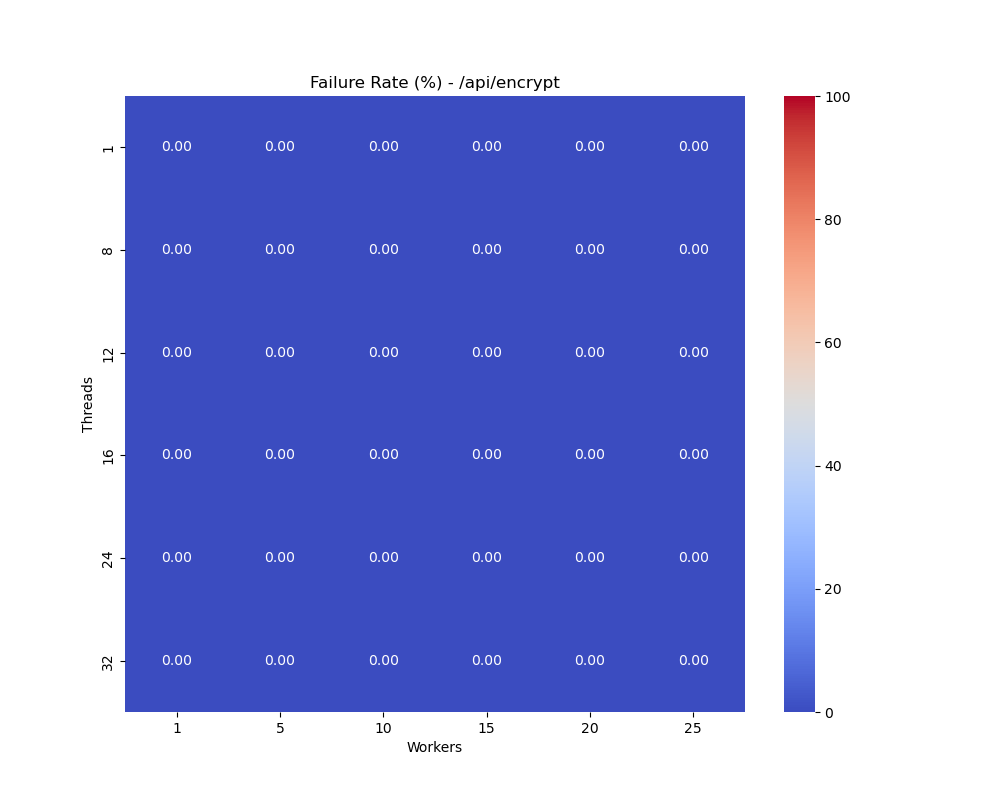
\includegraphics[width=\textwidth]{images/phase1/failure_rate__api_encrypt.png}
        %         \caption{Failure rate for /api/encrypt for different configurations of threads and workers}
        %         \label{fig:failurerateencrypt}
        %     \end{figure}

        %     \begin{figure}[h]
        %         \centering
        %         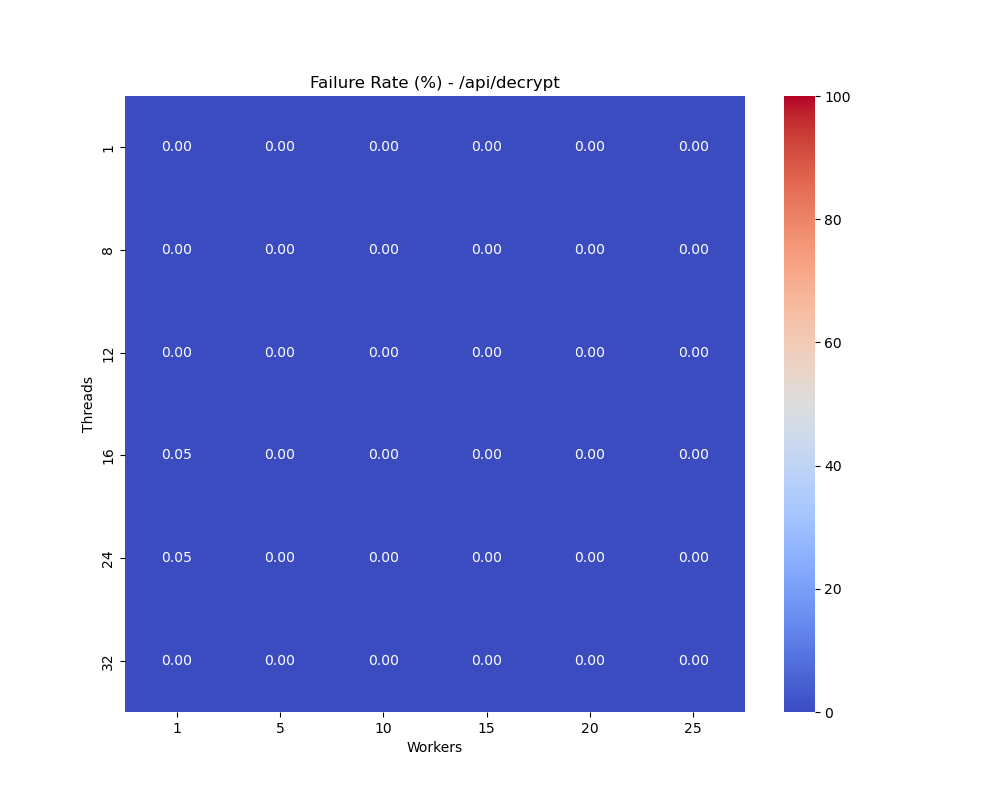
\includegraphics[width=\textwidth]{images/phase1/failure_rate__api_decrypt.png}
        %         \caption{Failure rate for /api/decrypt for different configurations of threads and workers}
        %         \label{fig:failureratedecrypt}
        %     \end{figure}


        \subsection{Concurrency analysis}
        \label{subsec:phase1_concurrency}

        The first phase of our analysis aimed to determine the optimal configuration of Gunicorn workers and threads for concurrent request handling. We fixed the payload size at 1\,KB, the number of concurrent users at 100, and the number of attributes in the encryption policy at one. The number of threads and workers was varied according to Formula~\ref{form:numberthreadsworkers}.

        \begin{equation}
            \label{form:numberthreadsworkers}
            (\text{threads}, \text{workers}) \mid \text{threads} \in \{1, 8, 12, 16, 24, 32\}, \text{workers} \in \{1, 5, 10, 15, 20, 25\} 
        \end{equation}

        Figure~\ref{fig:encrypt_response_time_workers} and Figure~\ref{fig:decrypt_response_time_workers} shows the response time for encryption and decryption with a fixed number of workers while varying the number of threads. The results indicate a relatively stable median response time across thread counts, suggesting that the system does not benefit significantly from thread-level concurrency.

        Figure~\ref{fig:encrypt_response_time_threads} and Figure~\ref{fig:decrypt_response_time_threads}, in contrast, presents the effect of increasing the number of workers with a fixed thread count. The response time decreases exponentialy as more workers are added, showing that the system benefits from process-based concurrency.

        Based on these results, we adopted a configuration of 25 workers and 1 thread for the remaining test phases. This choice aligns with Gunicorn's recommendation\footnote{\url{https://docs.gunicorn.org/en/latest/design.html\#how-many-workers}} for the optimal number of workers, given by Equation~\ref{form:numberworkers}, where \texttt{cores} is the number of logical cores available. The request times for this configuration can be seen in Table~\ref{tab:response_times}.

        \begin{equation}
            \label{form:numberworkers}
            \text{workers} = (2 \times \text{cores}) + 1
        \end{equation}

        \begin{figure}
            \centering
            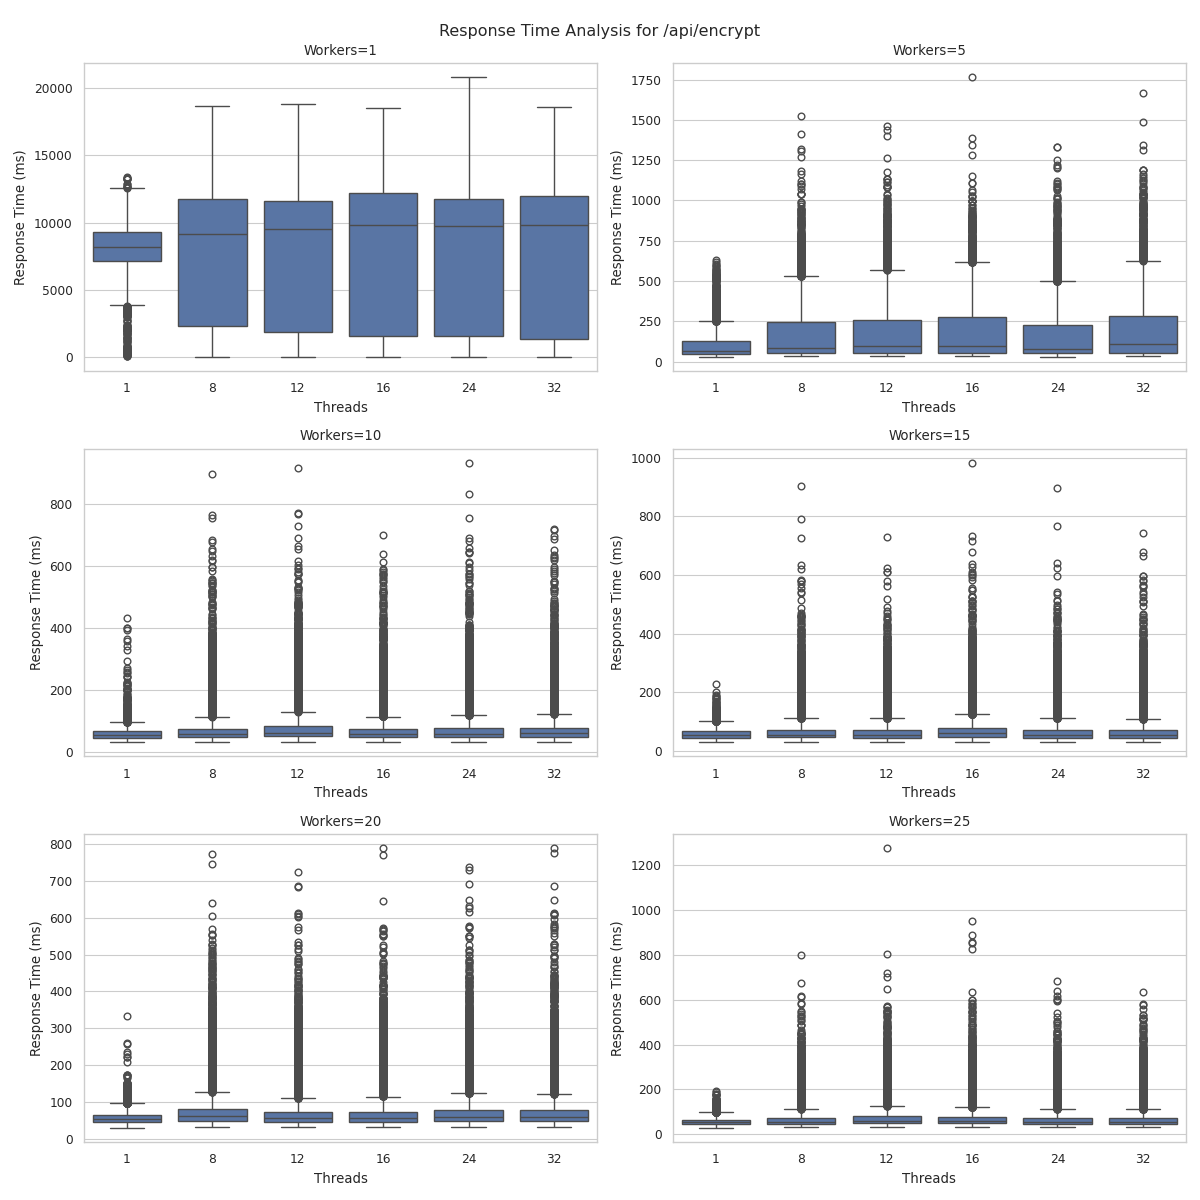
\includegraphics[width=\textwidth]{images/phase1/api_encrypt/response_time_workers_summary.png}
            \caption{Encryption response time varying the number of threads (workers fixed)}
            \label{fig:encrypt_response_time_workers}
        \end{figure}

        \begin{figure}
            \centering
            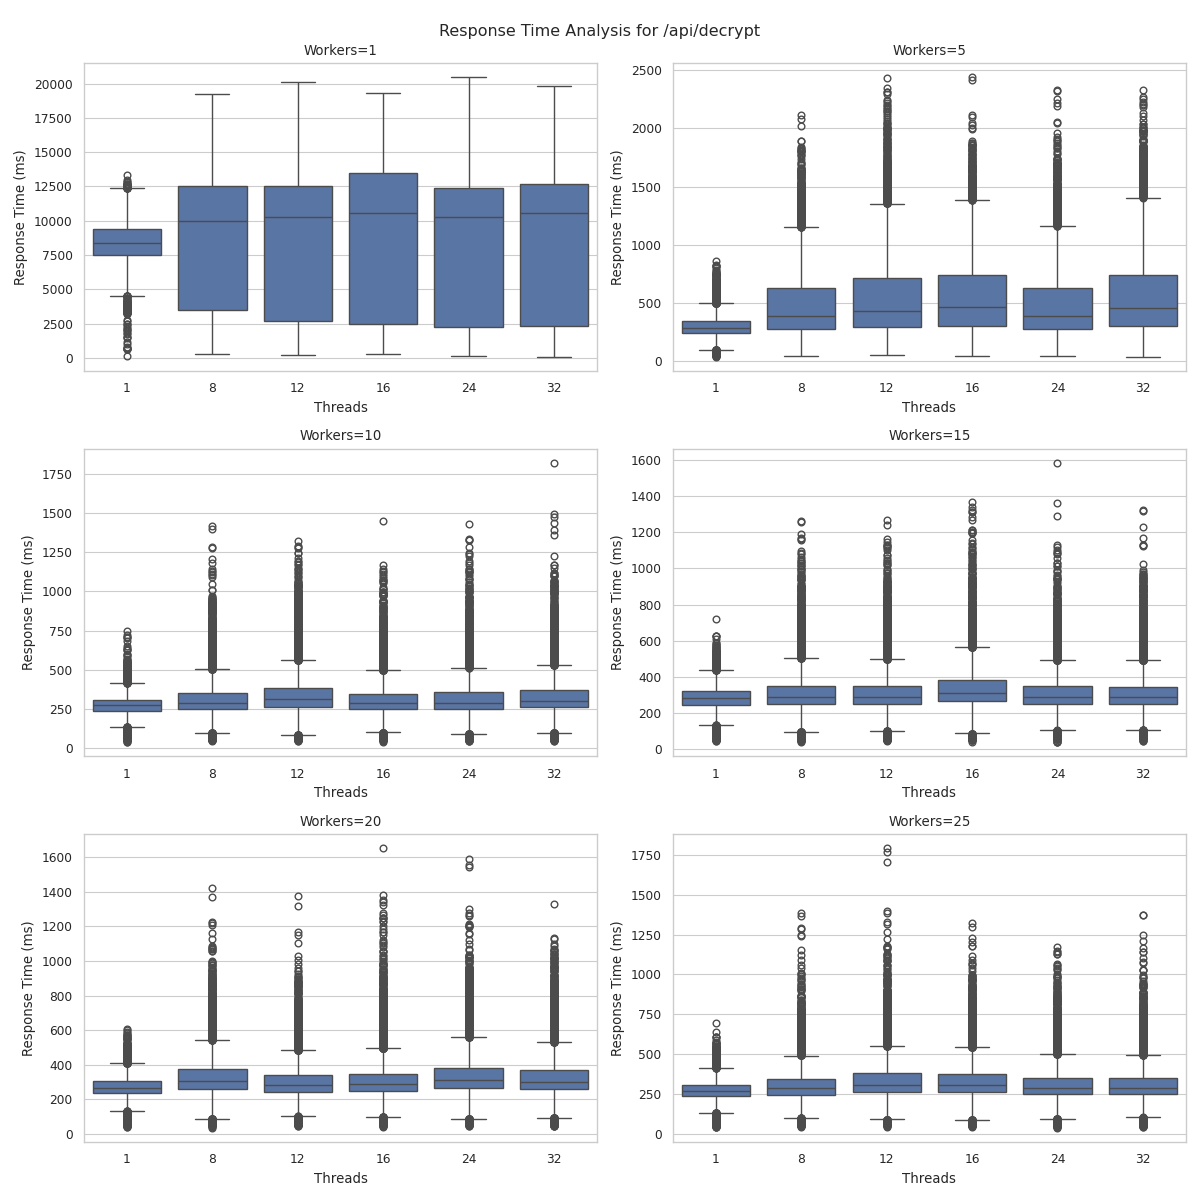
\includegraphics[width=\textwidth]{images/phase1/api_decrypt/response_time_workers_summary.png}
            \caption{Decryption response time varying the number of threads (workers fixed)}
            \label{fig:decrypt_response_time_workers}
        \end{figure}

        \begin{figure}
            \centering
            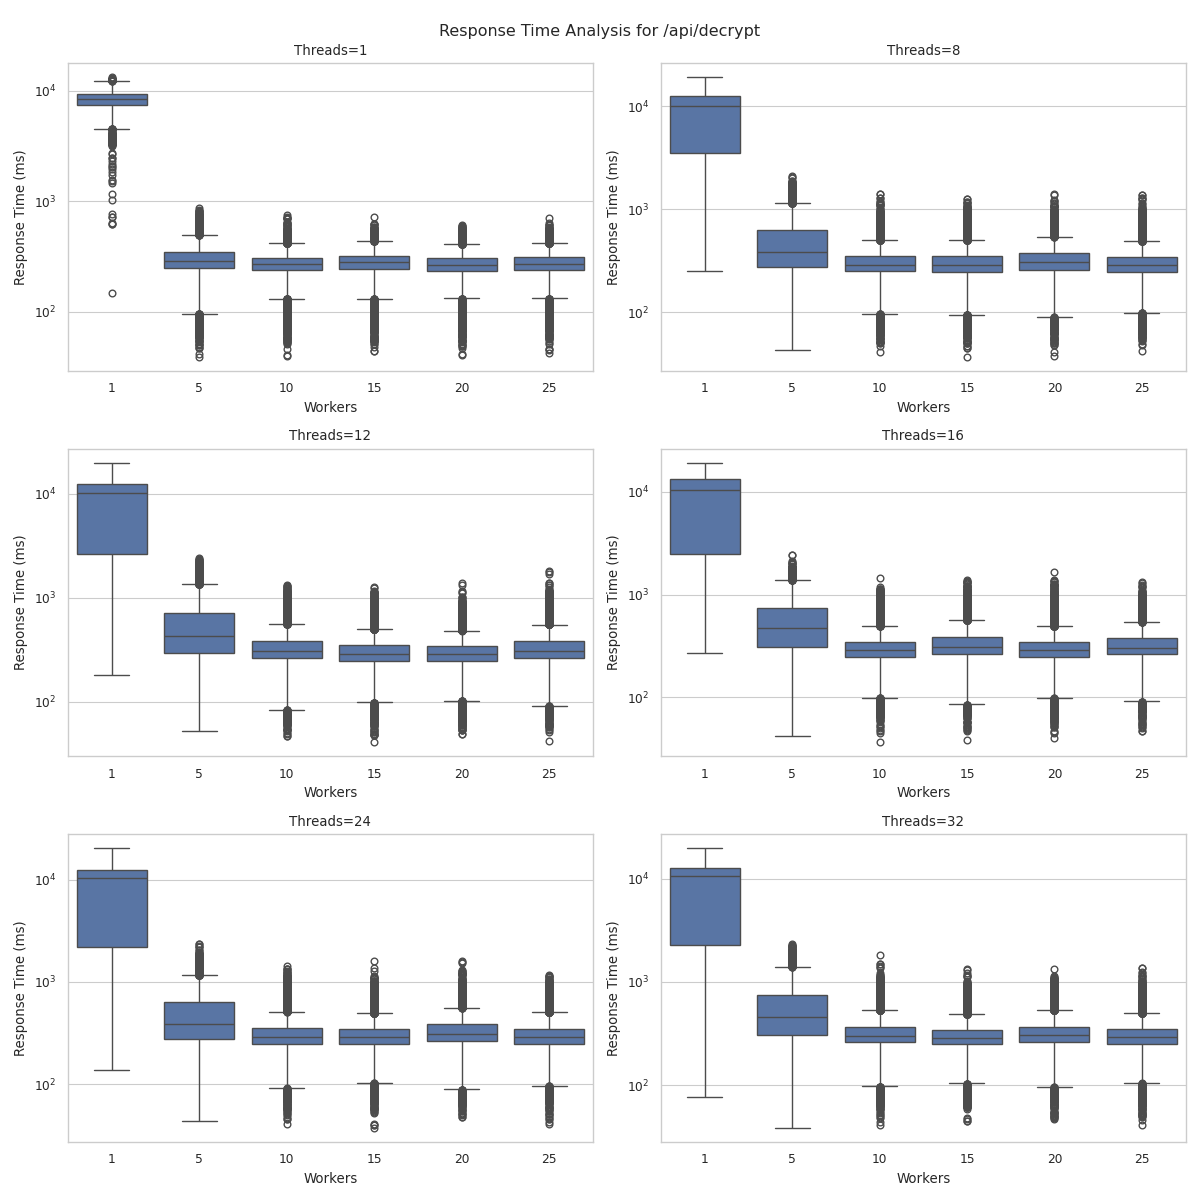
\includegraphics[width=\textwidth]{images/phase1/api_decrypt/response_time_threads_summary.png}
            \caption{Encryption response time varying the number of workers (threads fixed)}
            \label{fig:encrypt_response_time_threads}
        \end{figure}

        \begin{table}
                \centering
                \begin{tabular}{|l|l|l|l|l|}
                \hline
                    Endpoint & Mean Response Time (ms) & Std Dev (ms) & Total Requests & RPS \\ \hline
                    /api/decrypt & 273.51 & 71.38 & 7423 & 12.45 \\ \hline
                    /api/encrypt & 57.37 & 52.18 & 7539 & 12.59 \\ \hline
                \end{tabular}
                \caption{Summary of response times for encryption and decryption using 25 workers and 1 thread}
                \label{tab:response_times}
            \end{table}

        \begin{figure}
            \centering
            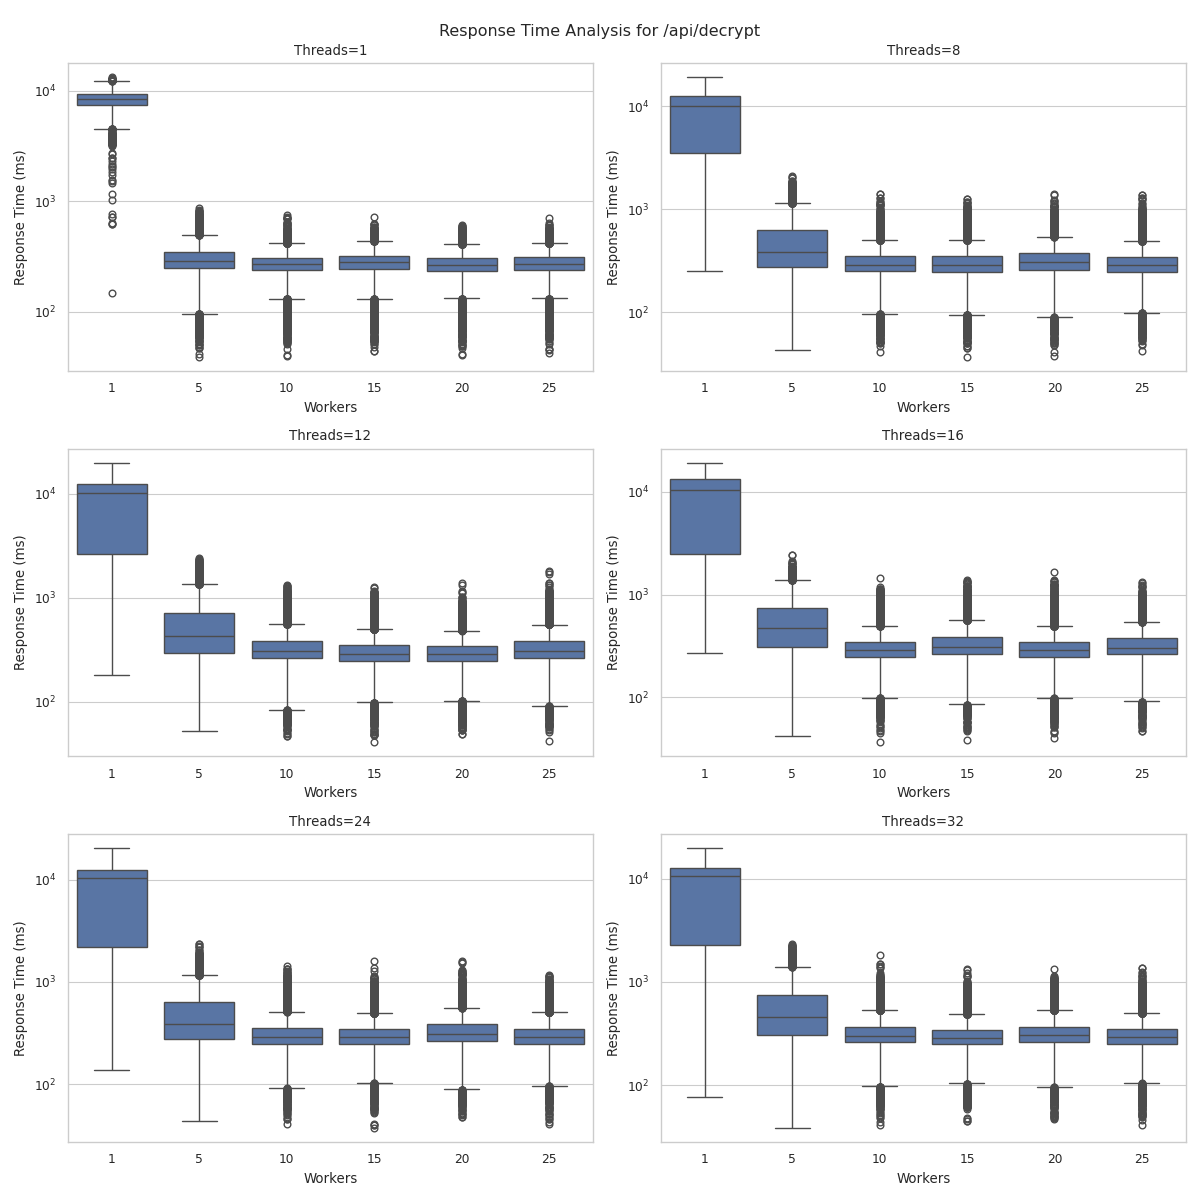
\includegraphics[width=\textwidth]{images/phase1/api_decrypt/response_time_threads_summary.png}
            \caption{Decryption response time varying the number of workers (threads fixed)}
            \label{fig:decrypt_response_time_threads}
        \end{figure}


        \subsection{Payload Size Impact Analysis}
        \label{subsec:phase2_payload}

            In the second phase, we evaluated the impact of payload size on the system's performance. The number of workers and threads was fixed at 25 and 1, respectively, and the number of users was kept at 100. The payload size was varied according to Formula~\ref{form:payloadsizes}.

            \begin{equation}
            \label{form:payloadsizes}
                \text{payload\_size} \in \{1\text{KB}, 4\text{KB}, 16\text{KB}, 32\text{KB}, 64\text{KB}, 256\text{KB}\}
            \end{equation}

            Figures~\ref{fig:encrypt_payload_size} and~\ref{fig:decrypt_payload_size} present the encryption and decryption response times, respectively, for different payload sizes. As expected, response time increases with larger payloads. However, the encryption process shows a more gradual increase compared to decryption, which may reflect higher complexity in the MA-ABE decryption routine. Table~\ref{tab:response_times} summarizes the mean response times and standard deviations for both encryption and decryption operations across all payload sizes. An original payload of 32KB expands to approximately 87KB, and a 256KB payload increases to about 699KB after encryption. This substantial expansion directly affects the storage requirements and bandwidth utilization for data retrieval from IPFS, especially crucial in resource-constrained hIoT environments where storage efficiency and network overhead are critical considerations. 
            

            \begin{figure}
                \centering
                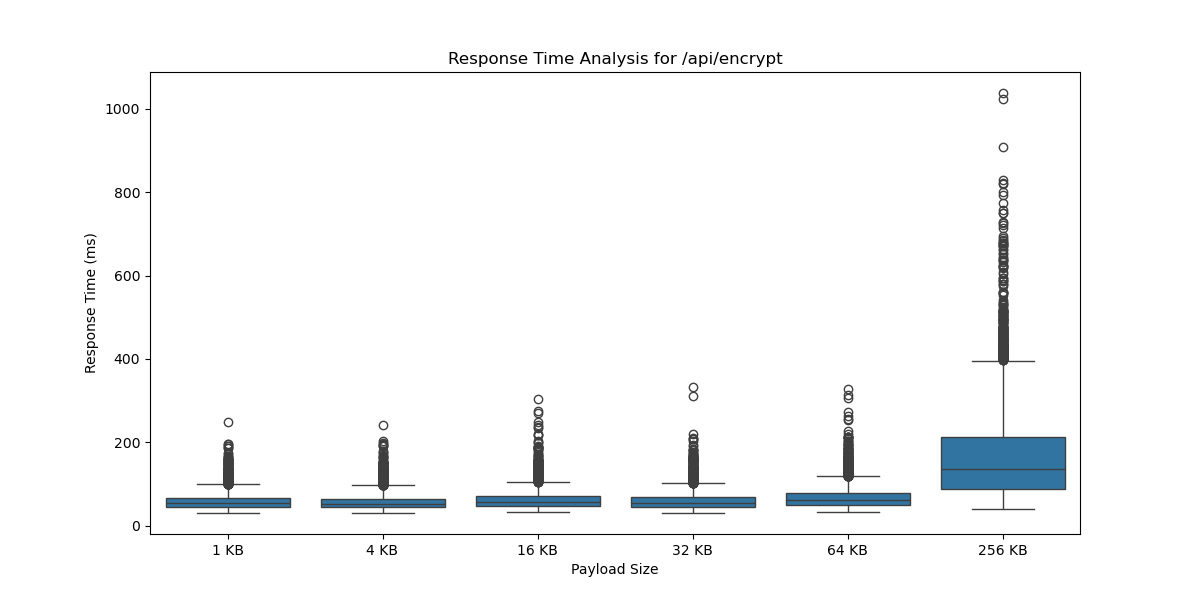
\includegraphics[width=\textwidth]{images/phase2/response_time_api_encrypt.png}
                \caption{Encryption response time for different payload sizes}
                \label{fig:encrypt_payload_size}
            \end{figure}

            \begin{figure}
                \centering
                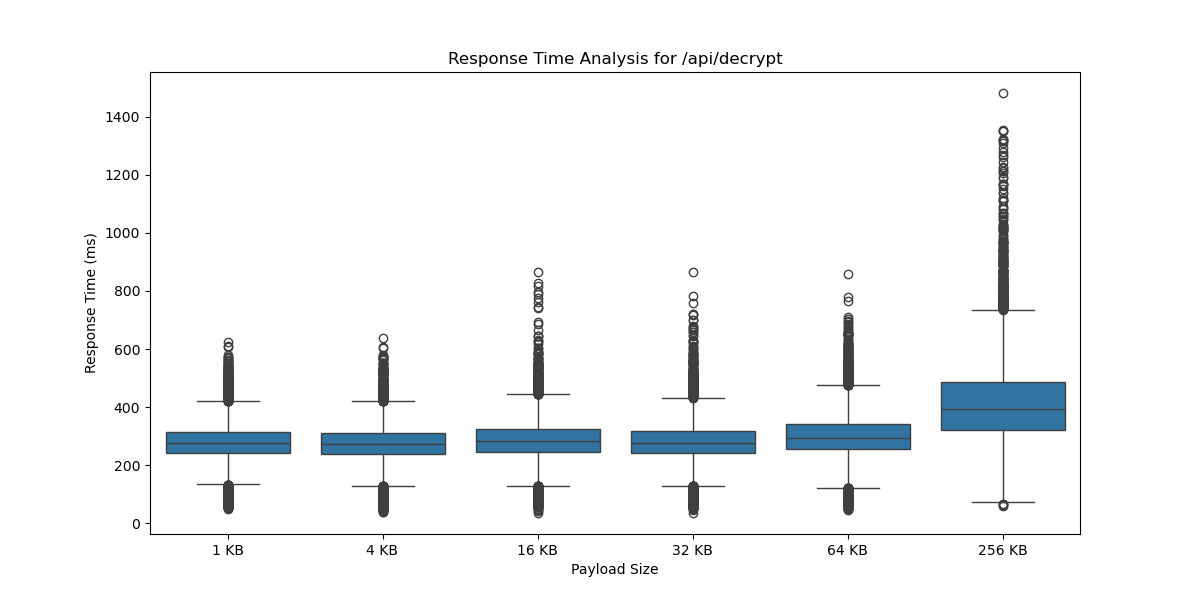
\includegraphics[width=\textwidth]{images/phase2/response_time_api_decrypt.png}
                \caption{Decryption response time for different payload sizes}
                \label{fig:decrypt_payload_size}
            \end{figure}

            \subsection{User Load Analysis}
            \label{subsec:user_load_analysis}

            To examine how the system scales with increasing numbers of concurrent users, we varied the number of users according to Formula~\ref{form:userload}. The payload size was fixed at 64\,KB (chosen based on the payload size analysis), and the number of workers and threads remained 25 and 1, respectively.

            \begin{equation}
            \label{form:userload}
                \text{users} \in \{10, 50, 100, 250, 500, 1000\}
            \end{equation}

            Figures~\ref{fig:encrypt_user_load} and~\ref{fig:decrypt_user_load} illustrate the effect of user load on response time. As expected, response time increases as more users are introduced. The system handles moderate user loads well, but performance degradation becomes more pronounced at the highest concurrency levels.

            \begin{figure}
                \centering
                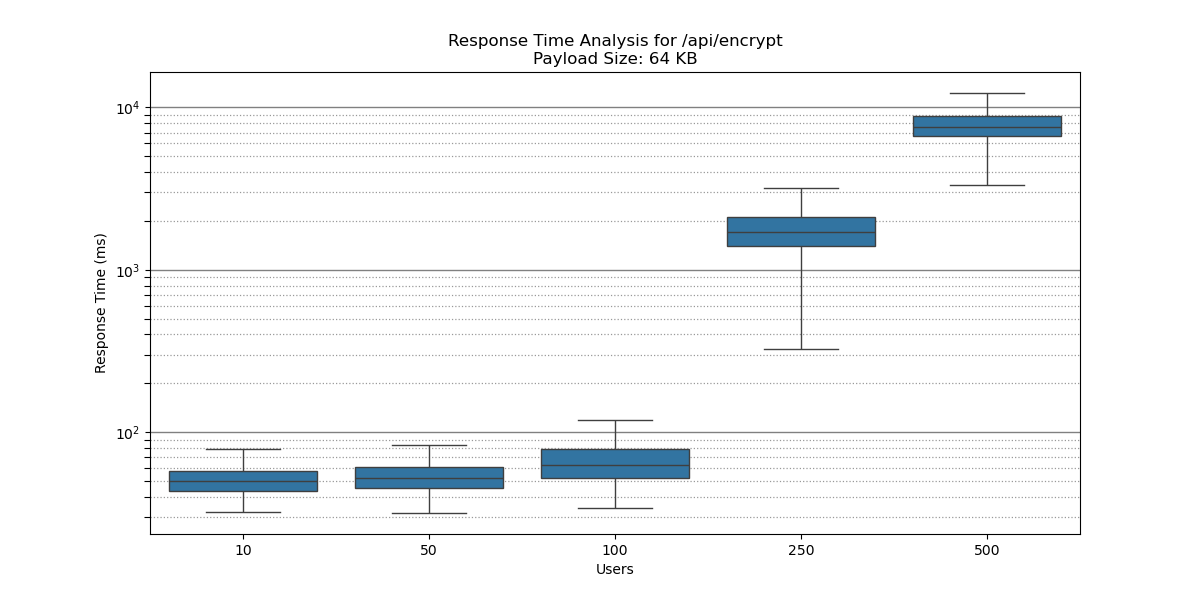
\includegraphics[width=\textwidth]{images/phase3/response_time_api_encrypt_64KB.png}
                \caption{Encryption response time for different user loads}
                \label{fig:encrypt_user_load}
            \end{figure}

            \begin{figure}
                \centering
                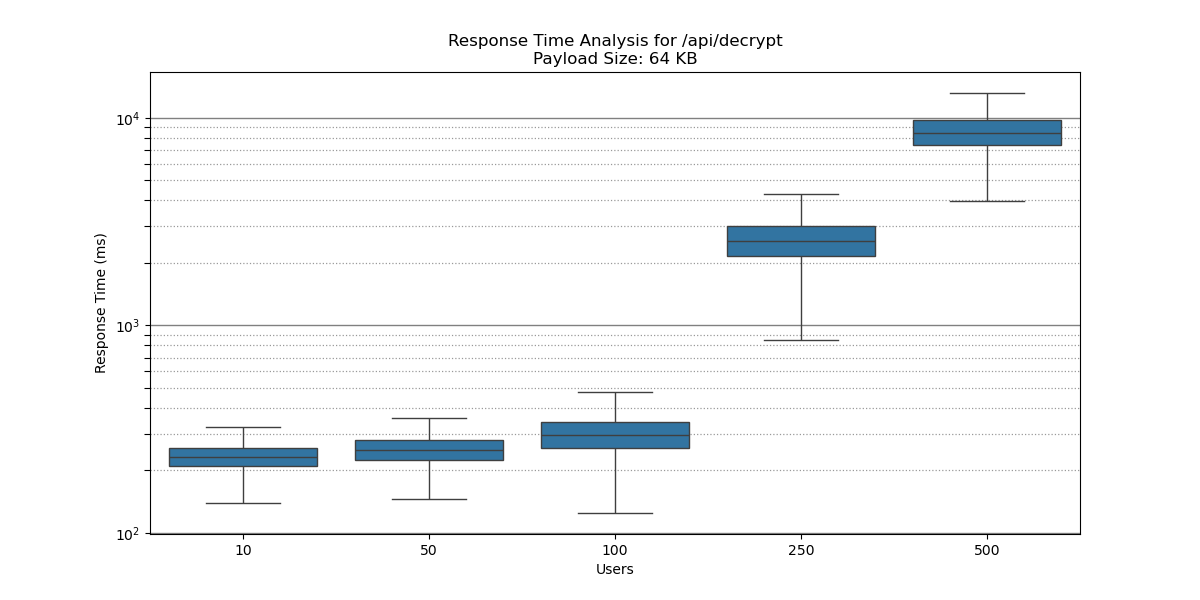
\includegraphics[width=\textwidth]{images/phase3/response_time_api_decrypt_64KB.png}
                \caption{Decryption response time for different user loads}
                \label{fig:decrypt_user_load}
            \end{figure}

            \subsection{Encryption Policy Size Analysis}
        \label{subsec:encryption_policy_size_analysis}

            To assess how the size of the encryption policy affects performance, we varied the number of attributes in the access policy from 1 to 10. The other parameters (payload size = 64\,KB, users = 100, workers = 25, threads = 1) were kept fixed.

            Figures~\ref{fig:encrypt_policy_size} and~\ref{fig:decrypt_policy_size} show how increasing the number of attributes in the policy affects encryption and decryption times. As expected, more complex policies result in higher response times due to the additional computational overhead involved in evaluating attribute trees and pairing operations.

            \begin{figure}
                \centering
                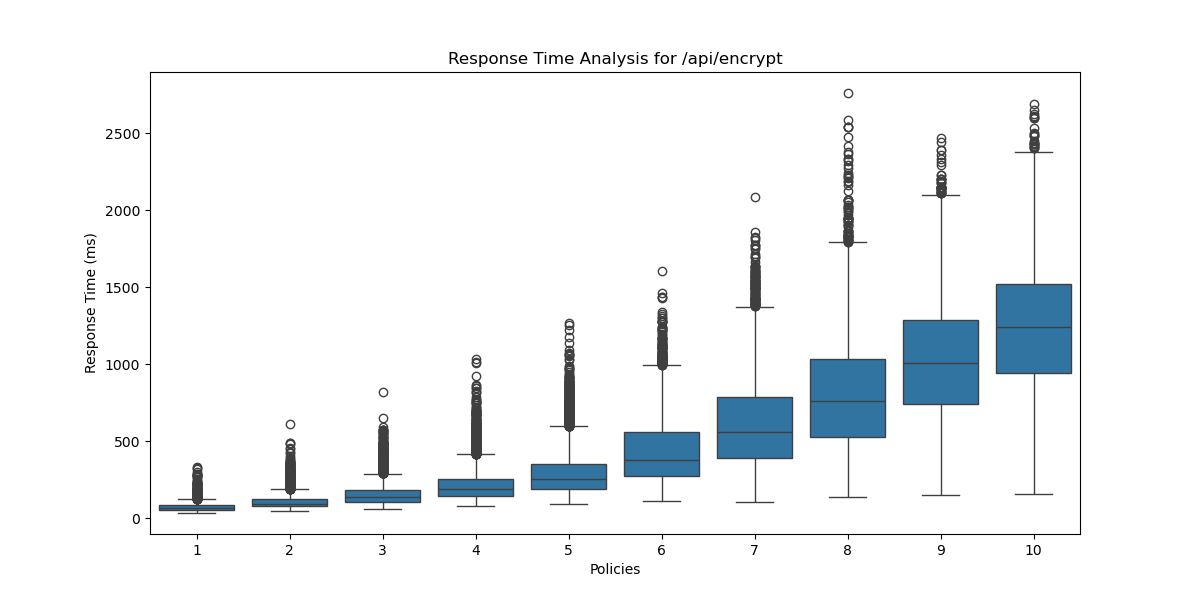
\includegraphics[width=\textwidth]{images/phase4/response_time_api_encrypt.png}
                \caption{Encryption response time for different policy sizes}
                \label{fig:encrypt_policy_size}
            \end{figure}

            \begin{figure}
                \centering
                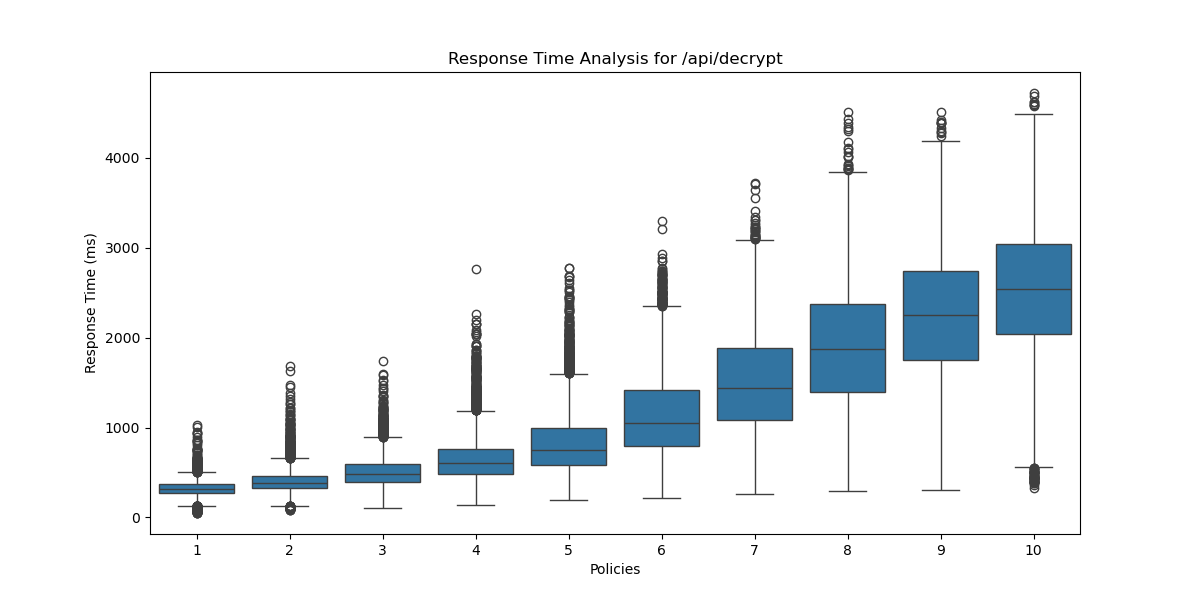
\includegraphics[width=\textwidth]{images/phase4/response_time_api_decrypt.png}
                \caption{Decryption response time for different policy sizes}
                \label{fig:decrypt_policy_size}
            \end{figure}

        
        \section{User key size}
            \label{sec:keysize}
            Figure~\ref{fig:user_key_size} shows the size of the user key for different number of attributes. The user key size increases linearly, reaching 25KB for 100 attributes.

            The evaluation of user key size reveals a linear correlation with the number of attributes assigned to a user, as illustrated in Figure~\ref{fig:user_key_size}. For instance, a user key can reach approximately 25KB for 100 attributes. This characteristic has significant implications for the overall storage footprint within the InterPlanetary File System (IPFS) architecture proposed by \citet{laura2023}. In her framework, data payloads are stored in IPFS blocks, and while our cryptographic scheme primarily encrypts the symmetric key rather than the entire payload with MA-ABE, the original payload itself also undergoes encryption with AES, and is then coupled with the encrypted symmetric key. This process introduces a measurable overhead to the size of the data being stored on IPFS. This highlights a fundamental trade-off: the enhanced security and fine-grained access control offered by our hybrid cryptographic scheme come with an increased burden on storage resources, necessitating further optimization strategies for highly constrained deployments.

            \ToDo{Fazer paralelo com trabalho da Laura e mostrar impacto da criptografia no armazenamento do payload nos blocos do IPFS}

            \begin{figure}
                \centering
                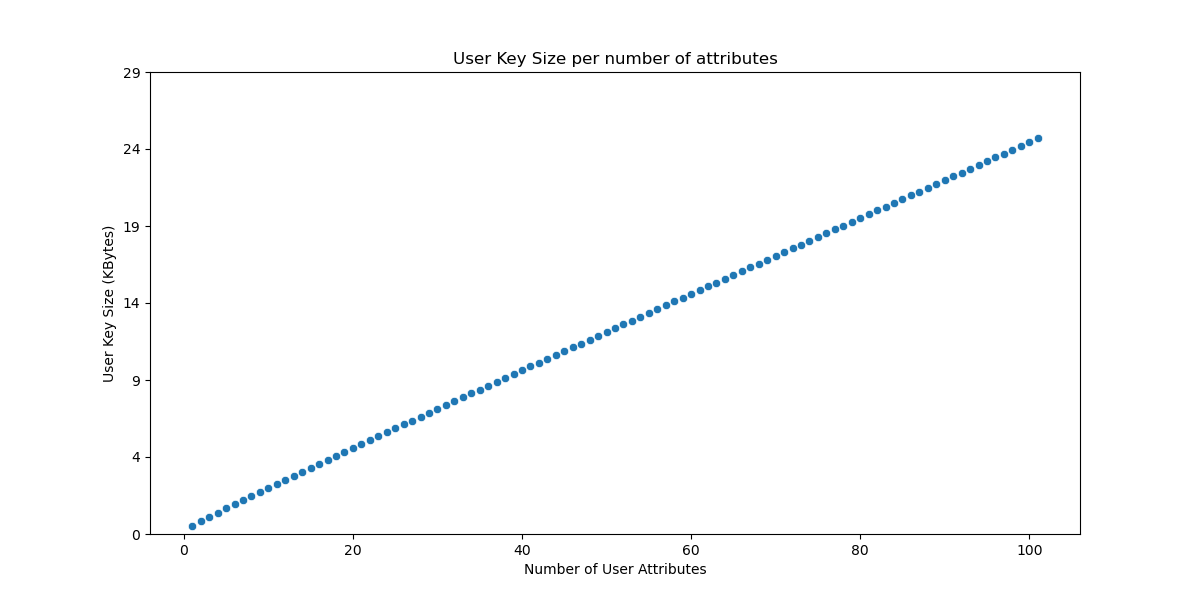
\includegraphics[width=\textwidth]{images/key_size_analysis/user_key_size_analysis.png}
                \caption{Comparison of user key size for different number of attributes}
                \label{fig:user_key_size}
            \end{figure}


        \section{Discussion}
            \label{sec:discussion}
            Ficou tudo uma bosta e não deu certo pq...

            Falar sobre o multi-thread e pq não funcionou. (evitar sincericídio)

            Charm crypto compila a parte de matematica da curva e faz load em um .so. Talvez isso seja a causa das falhas com multiplas threads

            Meu trabalho é maravilhoso pq resolve o gap da literatura

\Laura{olhar related works seção 3.3}

\chapter{Conclusion}
    \label{chap:conclusion}

    \section{Future Work}
        \label{sec:futurework}
        Latencia com a criptografia integrada ao framework da laura

        Tempo pra buscar chaves

        Alternativas para armazenamento das chaves, tonarnando a aplicação mais cpu bound

        Implementaion in a true distributed environment with multiple nodes


\bibliographystyle{abntex2-alf}
\bibliography{biblio}

\end{document}
